%
%===============>>  ГРУППА 10-1 МОДУЛЬ 8  <<=============
%
\setmodule{8}

%BEGIN_FOLD % ====>>_____ Занятие 1 _____<<====
\begin{class}[number=1]
	\begin{listofex}
		\item Вычислить с помощью метода приведения:
		\[ \sin135\degree;\;\cos240\degree;\;\tg150\degree;\;\ctg220\degree;\;\sin(-220\degree);\;\tg840\degree;\;\cos(-240\degree);\;\sin315\degree \]
		\item Вычислить:
		\begin{tasks}(1)
			\task \( \dfrac{\sqrt{3}}{\sin60\degree}+\dfrac{3}{\sin30\degree} \)
			\task \( \dfrac{17\sin155\degree}{\sin25\degree} \)
			\task \( \dfrac{-2\sin105\degree}{\cos15\degree} \)
			\task \( \sin^215\degree-1+\cos^215 \)
			\task \( -\sqrt{27}\cos30\degree-\sqrt{2}\sin45\degree\ctg60\degree\tg60\degree\)
		\end{tasks}
		\item Вычислить с помощью метода приведения:
		\[ \cos\dfrac{5\pi}{4};\;\sin\dfrac{7\pi}{3};\;\sin\dfrac{3\pi}{2};\;\sin\left( -\dfrac{5\pi}{3} \right);\;\cos\dfrac{7\pi}{6};\;\sin\dfrac{13\pi}{4};\;\sin\left( -\dfrac{7\pi}{6}  \right);\;\cos\dfrac{21\pi}{4} \]
		\item Вычислить:
		\begin{tasks}(2)
			\task \( \dfrac{5\cos29\degree}{\sin61\degree} \)
			\task \( -4\sqrt{3}\cos(-750\degree) \)
			\task \( \dfrac{4\cos146\degree}{\cos34\degree} \)
			\task \( 7\tg13\degree\cdot\tg77\degree \)
			\task \( \dfrac{12}{\sin^227\degree+\cos^2207\degree} \)
			\task \( \dfrac{5\sin98\degree}{\sin49\degree\cdot\sin41\degree} \)
			\task \( -50\tg9\degree\cdot\tg81\degree+31 \)
		\end{tasks}
		\item Найти:
		\begin{tasks}(1)
			\task \( 5\sin\alpha \), \quad если \( \cos\alpha=\dfrac{2\sqrt{6}}{5} \) и \( \alpha\in\left( \dfrac{3\pi}{2}; 2\pi \right) \);
			\task \( 3\cos\alpha \), \quad если \( \sin\alpha=-\dfrac{2\sqrt{2}}{3} \) и \( \alpha\in\left( \dfrac{3\pi}{2}; 2\pi \right) \);
			\task \( 24\cos\alpha \), \quad если \( \sin\alpha=-0,2 \);
			\task \( \sin\left( \dfrac{7\pi}{2}-\alpha \right) \), \quad если \( \sin\alpha=0,8 \) и \( \alpha\in\left( \dfrac{\pi}{2}; \pi \right) \);
		\end{tasks}
	\end{listofex}
\end{class}
%END_FOLD

%BEGIN_FOLD % ====>>_____ Занятие 2 _____<<====
\begin{class}[number=2]
	\begin{listofex}
		\item Найти:
		\begin{tasks}(2)
			\task \( \cos^2(-46\degree)+\sin^2(-46\degree) \)
			\task \( \sin^223\degree+9+\cos^223\degree \)
			\task \( \dfrac{-13\sin126\degree}{\sin54\degree} \)
			\task \( \dfrac{2\sin^221\degree+2\cos^221\degree}{4} \)
			\task \( \dfrac{ 12\sin 11 \degree \cdot \cos 11 \degree }{ \sin 22 \degree } \)
			\task \( \dfrac{ 24 (\sin^2 17 \degree-\cos^217 \degree) }{ \cos 34 \degree } \)
			\task \( \dfrac{ 5 \cos 29 \degree }{ \sin 61 \degree } \)
			\task \( 36 \sqrt{6} \tg \dfrac{ \pi }{ 4 } \sin \dfrac{ \pi }{ 4 } \)
			\task \( 4 \sqrt{2} \cos \dfrac{ \pi }{ 4 } \cos \dfrac{ 7\pi }{3  } \)
			\task \( \dfrac{ 8 }{ \sin \left( \dfrac{ -27\pi }{ 4 } \right) \cos \left( \dfrac{ 31\pi }{ 4 } \right) } \)
		\end{tasks}
		\item Вычислите:
		\begin{tasks}
			%\task \( \tg\alpha \), \quad если \( \dfrac{7\sin\alpha+13\cos\alpha}{5\sin\alpha-17\cos\alpha}=3 \).
			\task \( 5\sin\alpha \), если \( \cos\alpha=\dfrac{2\sqrt{6}}{5} \) и \( \alpha\in\left( \dfrac{3\pi}{2}; 2\pi \right) \);
			\task \( 3\cos\alpha \), если \( \sin\alpha=-\dfrac{2\sqrt{2}}{3} \) и \( \alpha\in\left( \dfrac{3\pi}{2}; 2\pi \right) \);
			\task \( 24\cos\alpha \), если \( \sin\alpha=-0,2 \);
			\task \( \sin\left( \dfrac{7\pi}{2}-\alpha \right) \), если \( \sin\alpha=0,8 \) и \( \alpha\in\left( \dfrac{\pi}{2}; \pi \right) \);
			%\task \( \dfrac{3\cos\alpha-4\sin\alpha}{2\sin\alpha-5\cos\alpha} \), если \( \tg\alpha=3 \).
		\end{tasks}
		%n5 cos1
		\item Найдите корни уравнения: \( \cos \dfrac{ \pi(x-7) }{ 3 } = 0,5 \).  В ответ запишите наибольший отрицательный корень.
		%n5 cos3
		\item Найдите корни уравнения: \( \cos \dfrac{ \pi(2x+9) }{ 3 } = \dfrac{ \sqrt{2} }{ 2 } \).  В ответ запишите наибольший отрицательный корень.
		%n5 tg1
		\item Найдите корни уравнения: \( \tg \dfrac{ \pi x }{ 4 } = -1 \).  В ответ запишите наибольший отрицательный корень.
		%n5 tg2
		\item Найдите корни уравнения: \( \tg \dfrac{ \pi (x+2) }{ 3 } = -\sqrt{3} \).  В ответ запишите наибольший отрицательный корень.
		%n5 sin1
		\item Найдите корни уравнения: \( \sin \dfrac{ \pi x }{ 3 } = 0,5 \).  В ответ запишите наименьший положительный корень.
	\end{listofex}
\end{class}
%END_FOLD

%BEGIN_FOLD % ====>>_ Домашняя работа 1 _<<====
\begin{homework}[number=1]
	\begin{listofex}
		\item Вычислить: %ПРОВЕРИТЬ НА ДУБЛИКАТЫ 111L1
		\begin{tasks}(2)
			\task \( \dfrac{5\cos29\degree}{\sin61\degree} \)
			\task \( -4\sqrt{3}\cos(-750\degree) \)
			\task \( \dfrac{4\cos146\degree}{\cos34\degree} \)
			\task \( 7\tg13\degree\cdot\tg77\degree \)
			\task \( \dfrac{12}{\sin^227\degree+\cos^2207\degree} \)
			\task \( \dfrac{5\sin98\degree}{\sin49\degree\cdot\sin41\degree} \)
			\task \( -50\tg9\degree\cdot\tg81\degree+31 \)
		\end{tasks}
		%n5 cos2
		\item Найдите корни уравнения: \( \cos \dfrac{ \pi(x-1) }{ 3 }=\dfrac{  1}{ 2 } \).  В ответ запишите наибольший отрицательный корень.
		%n5 sin2
		\item Найдите корни уравнения: \( \sin \dfrac{ \pi(4x-3) }{ 4 }=1 \).  В ответ запишите наибольший отрицательный корень.
		%n5 tg3
		%\item Найдите корни уравнения: \( \tg \dfrac{ \pi(x-3) }{ 6 }=\dfrac{ 1 }{ \sqrt{3} } \).  В ответ запишите наибольший отрицательный корень.
		\item Найдите: %6 1-6 9
		\begin{tasks}
			\task \( \tg \alpha \), если \( \cos \alpha = \dfrac{ \sqrt{10} }{ 10 } \) и \( \alpha\in\left( \dfrac{ 3\pi }{ 2 };2\pi \right) \);
			\task \( 26 \cos \left( \dfrac{ 3\pi }{ 2 }+\alpha \right) \), если \( \cos \alpha = \dfrac{ 12 }{ 13 } \) и \( \alpha\in\left( \dfrac{ 3\pi }{ 2 };2\pi \right) \);
			%\task \( \dfrac{ 10\sin 6 \alpha }{ 3 \cos 3 \alpha } \), если \( \sin 3 \alpha = 0,6 \).
		\end{tasks}
	\end{listofex}
\end{homework}
%END_FOLD

%BEGIN_FOLD % ====>>_____ Занятие 3 _____<<====
\begin{class}[number=3]
	\begin{listofex}
			\item Вычислите: %111
		\begin{tasks}(2)
			\task \( \dfrac{ 5\sin 74 \degree }{ \cos 37 \degree \cdot \cos 53 \degree } \)
			\task \( \dfrac{ 23 }{ \sin^2 56 \degree + 1 + \sin^2 146 \degree } \)
			\task \( -\dfrac{ 4 }{ \sin^2 27 \degree + \sin^2 117 \degree } \)
			\task \( -\dfrac{ 4\cos 22,5 \degree \sin 22,5 \degree }{ 8 } \)
			\task \( \dfrac{ 50 \sin 19 \degree \cos 19 \degree }{ \sin 38 \degree } \)
			\task \( \dfrac{ \sin \dfrac{ 3\pi }{8 } \cos \dfrac{ 3\pi }{ 8 } }{ 20 } \)
			\task \( -\dfrac{ 7 }{ \sin^2 \left( \dfrac{ \pi }{ 15 } \right) + \cos^2 \left( \dfrac{ \pi }{ 15 } \right) } \)
			\task \( \cos^2\left( -\dfrac{ 3\pi }{ 8 } \right) +\sin^2\left( -\dfrac{ 3\pi }{ 8 } \right) \)
			\task \( \sin^2 (-88\degree) + \cos^2 (-88\degree) -5 \)
			\task \( \dfrac{2\sin^2 21\degree+2\cos^221\degree}{4} \)
		\end{tasks}
		%\item Найдите: %111
		%\begin{tasks}
		%	\task \( \dfrac{ 10\sin 6 \alpha }{ 3 \cos 3 \alpha } \), если \( \sin 3 \alpha = 0,6 \).
		%\end{tasks}
		%n5 cos1
		\item Найдите корни уравнения: \( \cos \dfrac{ \pi(x-7) }{ 3 } = 0,5 \).  В ответ запишите наибольший отрицательный корень.
		%n5 cos3
		\item Найдите корни уравнения: \( \cos \dfrac{ \pi(2x+9) }{ 3 } = \dfrac{ \sqrt{2} }{ 2 } \).  В ответ запишите наибольший отрицательный корень.
		%n5 tg1
		\item Найдите корни уравнения: \( \tg \dfrac{ \pi x }{ 4 } = -1 \).  В ответ запишите наибольший отрицательный корень.
		%n5 tg2
		\item Найдите корни уравнения: \( \tg \dfrac{ \pi (x+2) }{ 3 } = -\sqrt{3} \).  В ответ запишите наибольший отрицательный корень.
		%n5 sin1
		\item Найдите корни уравнения: \( \sin \dfrac{ \pi x }{ 3 } = 0,5 \).  В ответ запишите наименьший положительный корень.
	\end{listofex}
\end{class}
%END_FOLD

%BEGIN_FOLD % ====>>_____ Занятие 4 _____<<====
\begin{class}[number=4]
	\begin{listofex}
		%n5 cos2
		\item Найдите корень уравнения: \( \cos \dfrac{ \pi(x-1) }{ 3 }=\dfrac{ 1 }{ 2 } \). В ответе запишите наибольший отрицательный корень.
		%n5 cos4
		\item Найдите корень уравнения: \( \cos \dfrac{ \pi(x+1) }{ 4 }=\dfrac{ \sqrt{2} }{ 2 } \). В ответе запишите наименьший положительный корень
		%n5 tg3
		\item Решите уравнение \(\tg \dfrac{ \pi(x-3) }{ 6 }= \dfrac{ 1 }{ \sqrt{3} }\). В ответе напишите наибольший отрицательный корень.
		%n5 tg4
		\item Решите уравнение \(\tg \dfrac{ \pi(4x-5) }{4 }= -1\). В ответе напишите наименьший положительный корень.
		%n5 sin2
		\item Решите уравнение \( \sin \dfrac{ \pi(4x-3) }{ 4 }=1 \). В ответе напишите наибольший отрицательный корень.
		%n5 sin3
		\item Решите уравнение \( \sin \dfrac{ \pi(8x+3) }{ 6 }=0,5 \). В ответе напишите наименьший положительный корень.
		%priklad trigon 1
		\item При нормальном падении света с длиной волны \( \lambda=400 \) нм на дифракционную решeтку с периодом \(d\) нм наблюдают серию дифракционных максимумов. При этом угол \(\varphi\)  (отсчитываемый от перпендикуляра к решeтке), под которым наблюдается максимум, и номер максимума \(k\) связаны соотношением \(d \sin \varphi= k\lambda\). Под каким минимальным углом \(\varphi\) (в градусах) можно наблюдать второй максимум на решeтке с периодом, не превосходящим \(1600\) нм?
		%priklad trigon 2
		\item Два тела массой \(m=2\) кг каждое, движутся с одинаковой скоростью  \(v =10\) м/с под углом \(2\alpha\) друг к другу. Энергия (в джоулях), выделяющаяся при их абсолютно неупругом соударении определяется выражением \(Q= m v^2 \sin^2 \alpha \). Под каким наименьшим углом \(2\alpha\) (в градусах) должны двигаться тела, чтобы в результате соударения выделилось не менее \(50\) джоулей?
		\item Найдите площадь треугольника, две стороны которого равны \(8\) и \(12\), а угол между ними равен \(30 \degree\).
		\item Большее основание равнобедренной трапеции равно \(34\). Боковая сторона равна \(14\). Синус острого угла равен \( \dfrac{ 2\sqrt{10}}{ 7 } \). Найдите меньшее основание.
		\item Основания равнобедренной трапеции равны \(7\) и \(51\). Тангенс острого угла равен \( \dfrac{ 5 }{ 11 } \).  Найдите высоту трапеции.
	\end{listofex}
\end{class}
%END_FOLD

%BEGIN_FOLD % ====>>_ Домашняя работа 2 _<<====
\begin{homework}[number=2]
	\begin{listofex}
		%n5 cos5
		\item Найдите корень уравнения: \( \cos \dfrac{ \pi(8x+1) }{ 6 } = \dfrac{ \sqrt{3} }{ 2 } \). В ответе запишите наибольший отрицательный корень.
		%n5 tg5
		\item Решите уравнение \( \tg \dfrac{ \pi(x+3) }{ 3 }=-\sqrt{3} \). В ответе напишите наибольший отрицательный корень.
		%n5 sin4
		\item Решите уравнение \( \sin \dfrac{ \pi(x+9) }{ 4 }=-\dfrac{ \sqrt{2} }{ 2 } \). В ответе напишите наименьший положительный корень.
		%priklad trigon 3
		\item Катер должен пересечь реку шириной \(L = 100\) м и со скоростью течения \(u =0,5\) м/с так, чтобы причалить точно напротив места отправления. Он может двигаться с разными скоростями, при этом время в пути, измеряемое в секундах, определяется выражением \(t=\dfrac{ L }{ u } \ctg \alpha \) где \(\alpha\) --- острый угол, задающий направление его движения (отсчитывается от берега). Под каким минимальным углом \(\alpha\) (в градусах) нужно плыть, чтобы время в пути было не больше \(200\) с?
		%трапеция N5
		\item Меньшее основание равнобедренной трапеции равно \(23\). Высота трапеции равна \(39\). Тангенс острого угла равен \(\dfrac{ 13 }{ 8 }\). Найдите большее основание.
		%треуг1 N5
		\item В треугольнике \(ABC\): \(AC=BC=7, \tg A = \dfrac{ 33 }{ 4\sqrt{33} }\). Найдите \(AB\).
		%параллелог1 N1
		\item В параллелограмме \(ABCD \): \( AB  =  3, AD  =  21\), \( \sin A = \dfrac{ 6 }{ 7 } \). Найдите большую высоту параллелограмма.
	\end{listofex}
\end{homework}
%END_FOLD

%BEGIN_FOLD % ====>>_____ Занятие 5 _____<<====
\begin{class}[number=5]
	\begin{listofex}
		\item В пачке \(250\) листов бумаги формата \(A4\). За неделю в офисе расходуется \(700\) листов. Какого наименьшего количества пачек бумаги хватит на \(8\) недель.
		\item Установите соответствие между величинами и их возможными значениями: к каждому элементу первого столбца подберите соответствующий элемент из второго столбца. \\ \\
		\begin{minipage}[t]{0.58\linewidth}
			\textbf{Величины:}
			\begin{tasks}
				\task площадь трехкомнатной квартиры
				\task площадь футбольного поля
				\task площадь территории России
				\task площадь купюры достоинством в \(100\) рублей \\
			\end{tasks}
		\end{minipage}
		\hspace{0.05\linewidth}
		\begin{minipage}[t]{\textwidth}
			\textbf{Возможные значения:}
			\begin{tasks}
				\task \( 0,7 \) га
				\task \( 100 \) кв. м
				\task \( 97,5 \) кв. см
				\task \( 17,1 \) млн кв. км
			\end{tasks}
		\end{minipage}
		\item На диаграмме показано количество посетителей сайта РИА «Новости» во все дни с \(10\) по \(29\) ноября \(2009\) года. По горизонтали указываются дни месяца, по вертикали --- количество посетителей сайта за данный день. Определите по диаграмме, какого числа количество посетителей сайта РИА «Новости» было наименьшим за указанный период.
		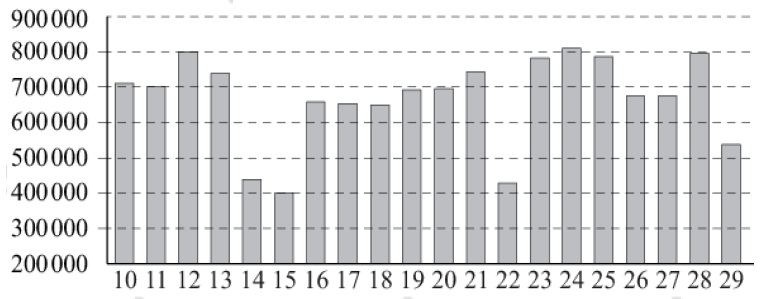
\includegraphics[align=t, width=\linewidth]{../pics/G101M8L5-1}
		\item Площадь четырехугольника можно вычислить по формуле \[S=\dfrac{ 1 }{ 2 }d_1 d_2 \sin \alpha,\] где \(d_1\) и \(d_2\) --- длины диагоналей четырехугольника, \(\alpha\) --- угол между диагоналями. Пользуясь этой формулой, найдите площадь \(S\), если \(d_1=4, d_2 = 7, \sin \alpha = \dfrac{  2}{ 7 }\).
		\item Научная конференция проводится в \(3\) дня. Всего запланировано \(50\) докладов: в первый день --- \(18\) докладов, остальные распределены поровну между днями. Порядок докладов определяется случайным образом. Какова вероятность того, что доклад профессора М. окажется запланированным на последний день конференции?
		\item Независимая экспертная лаборатория определяет рейтинг мясорубок на основе коэффициента ценности, равного \(0,01\) средней цены \(P\) (в рублях), показателей функиональности \(F\), качества \(Q\) и дизайна \(D\). Рейтинг \(R\) вычисляется по формуле: \[ R=3(F+1)+D-0,01P. \] В таблице даны цены и показатели четырех моделей мясорубок:
		\\
		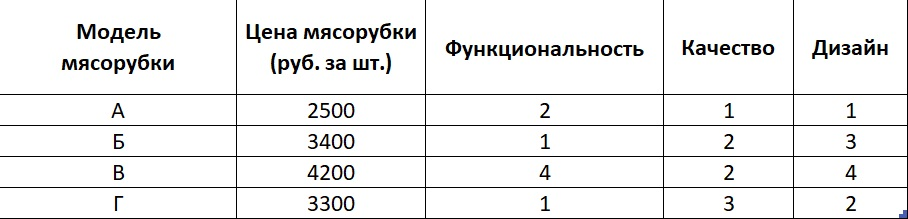
\includegraphics[align=t, width=\linewidth]{../pics/G101M8L5-2}
		\\
		\\ Найдите наивысший рейтинг мясорубки из представленных в таблице.
		\item На рисунках изображены графики функций вида \(y=kx+b\). Установите соответствие между графиками функций и угловыми коэффициентами прямых.
		\\ \textbf{Графики:}
		\\
		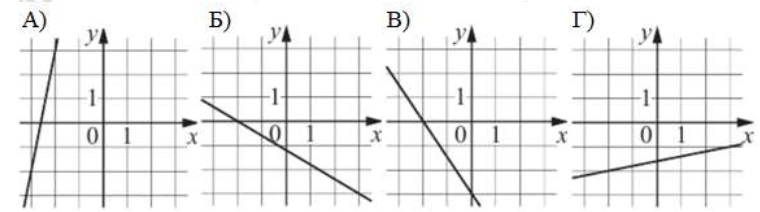
\includegraphics[align=t, width=\linewidth]{../pics/G101M8L5-3}
		\\ \\
		\textbf{Угловые коэффициенты:}
		\begin{tasks}(4)
			\task \( 0,2 \)
			\task \( 5 \)
			\task \( -1,5 \)
			\task \( -0,6 \)
		\end{tasks}
		\newpage
		\item В группе учится \(30\) студентов, из них \(20\) студентов получили зачет по экономике и \(20\) студентов получили зачет по английскому языку. Выберите утверждения, которые следуют из приведенных данных. В этой группе:
		\begin{tasks}
			\task не менее \(10\) студентов не получили зачета ни по экономике, ни по английскому языку
			\task хотя бы \(10\) студентов получили зачеты и по экономике, и по английскому языку
			\task не больше \(20\) студентов получили зачеты и по экономике, и по английскому языку
			\task найдется студент, который не получил зачета по английскому языку, но получил зачет по экономике.
		\end{tasks}
		\item
		\begin{minipage}[t]{\bodywidth}
			План местности разбит на клетки. Каждая клетка является квадратом размером \(1\)м на \(1\)м. Найдите площадь участка, изображенного на плане. Ответ дайте в квадратных метрах.
		\end{minipage}
		\hspace{0.02\linewidth}
		\begin{minipage}[t]{\picwidth}
			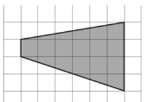
\includegraphics[align=t, width=\linewidth]{../pics/G101M8L5-4}
		\end{minipage}
		\item 
		\begin{minipage}[t]{\bodywidth}
			На рисунке показано, как выглядит колесо с \(7\) спицами. Сколько будет спиц в колесе, если угол между соседними спицами в нем будет равен \(20 \degree \)?
		\end{minipage}
		\hspace{0.02\linewidth}
		\begin{minipage}[t]{\picwidth}
			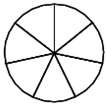
\includegraphics[align=t, width=\linewidth]{../pics/G101M8L5-5}
		\end{minipage}
		%11
		\item 
		\begin{minipage}[t]{\bodywidth}
			Плоскость, проходящая через точки \(A\), \(B\) и \(C\), разбивает куб на два многогранника. Сколько вершин у получившегося многогранника с большим числом граней?
		\end{minipage}
		\hspace{0.02\linewidth}
		\begin{minipage}[t]{\picwidth}
			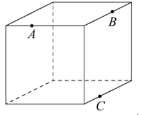
\includegraphics[align=t, width=\linewidth]{../pics/G101M8L5-6}
		\end{minipage}
		%12
		\item В прямоугольном треугольнике \(ABC\) внешний угол при вершине \(A\) равен \(120\degree \). Катет \(AC = 17\). Найдите гипотенузу \(AB\).
		%13
		\item 
		\begin{minipage}[t]{\bodywidth}
			В основании прямой призмы лежит прямоугольный треугольник, катеты которого равны \(3\) и \(16\). Найдите объем призмы, если ее высота равна \(3\).
		\end{minipage}
		\hspace{0.02\linewidth}
		\begin{minipage}[t]{\picwidth}
			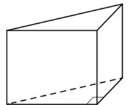
\includegraphics[align=t, width=\linewidth]{../pics/G101M8L5-7}
		\end{minipage}
		\item Найдите значение выражения: \( 4,1 \cdot 7,7 + 0,86 \)
		\item Товар на распродаже уценили на \(30\%\), при этом он стал стоить \(350\) рублей. Сколько рублей стоит товар до распродажи?
		\item Найдите значение выражения: \( (\sqrt{10}-2\sqrt{3})(\sqrt{10}+2\sqrt{3}) \)
		\item Найдите корень уравнения: \(3^{x-8}=\dfrac{ 1 }{ 9 }\)
		\item Каждому из четырѐх чисел в левом столбце соответствует отрезок, которому он принадлежит. Установите соответствие между числами и отрезками из правого столбца. \\ \\
		\begin{minipage}[t]{0.58\linewidth}
			\textbf{Числа:}
			\begin{tasks}
				\task \( \log_235 \)
				\task \( \dfrac{ 7 }{4  } \)
				\task \( \sqrt{13} \)
				\task \( 0,39^{-1} \)
			\end{tasks}
		\end{minipage}
		\hspace{0.05\linewidth}
		\begin{minipage}[t]{\textwidth}
			\textbf{Отрезки:}
			\begin{tasks}
				\task \( [1;2] \)
				\task \( [2;3] \)
				\task \( [3;4] \)
				\task \( [5;6] \)
			\end{tasks}
		\end{minipage}
		\item Найдите четырехзначное число, кратное \(88\), все цифры которого различны и четны. В ответе укажите какое-нибудь одно такое число.
		\item Первую треть трассы автомобиль ехал со скоростью \(60\) км/ч, вторую треть --- со скоростью \(120\) км/ч, а последнюю --- со скоростью \(110\) км/ч. Найдите среднюю скорость автомобиля на протяжении всего пути. Ответ дайте в км/ч.
		\item Петя меняет маленькие фишки на большие. За один обмен он получает \(3\) большие фишки, отдав \(10\) маленьких. До обменов у Пети было \(100\) фишек (среди них были и большие, и маленькие), а после стало \(65\). Сколько обменов он совершил?
	\end{listofex}
\end{class}
%END_FOLD

%BEGIN_FOLD % ====>>_____ Занятие 6 _____<<====
\begin{class}[number=6]
	\begin{listofex}
		\item Занятие 6
	\end{listofex}
\end{class}
%END_FOLD

%BEGIN_FOLD % ====>>_ Домашняя работа 3 _<<====
\begin{homework}[number=3]
	\begin{listofex}
		\item Домашняя работа 3
	\end{listofex}
\end{homework}
%END_FOLD

%BEGIN_FOLD % ====>>_____ Занятие 7 _____<<====
\begin{class}[number=7]
	\title{Подготовка к проверочной}
	\begin{listofex}
		\item Занятие 7
	\end{listofex}
\end{class}
%END_FOLD

=%BEGIN_FOLD % ====>>_ Проверочная работа _<<====
\begin{exam}
	\begin{listofex}
		\item Проверочная
	\end{listofex}
\end{exam}
%END_FOLD